%!TEX root = ./intern_report.tex

\subsection{Company Overview}

\paragraph{}
Wave Computing is a USA Silicon Valley based company that specializes in dataflow technology~\cite{waveintro}, an alternative to the tensorflow~\cite{tflow} technology used by tech giants such as {Nvidia} and {Google} to accelerate {AI} and neural net training. Although the company is relatively new to the game, they have had a number of notable achievements, which are explained below in detail. They outsource their design contracts to teams around the globe and one of these contracts was undertaken by Paraqum Technologies. This particular team works with the Software development kit ({SDK}) and the applications of the Wave dataflow platform.
\begin{figure}[h]
    \centering
    
\includegraphics[trim=0cm 0cm 0cm 0cm, clip=true,scale=1]{figures/wave_logo.png}
    \caption{Wave Computing logo\label{Fig:Wave}}\vspace{-4mm}
    \end{figure}


\paragraph{}
Paraqum Technologies is one of the very first truly Sri Lankan Electronics industry companies in the country. It undertakes Electronic design contracts from big companies from around the world such as Osprey video and of course, Wave Computing. They also have their own network product line. The company had one of their teams working on a design project of Wave Computing which split up in November 2018 to form the Sri Lankan branch of Wave Computing (pvt) Ltd. 
\begin{figure}[h]
    \centering
    
\includegraphics[trim=0cm 0cm 0cm 0cm, clip=true,scale=1]{figures/pqm_logo.png}
    \caption{Paraqum Technologies logo\label{Fig:Paraqum}}\vspace{-4mm}
    \end{figure}

\paragraph{}
My work was focused on the SDK layer of the Wave dataflow platform. This describes a large toolchain of software utilities that are the primary way that an advanced user would interact with the system. This team is also one of the busiest teams of the whole organization because of the sheer complexity of the SDK. In the context of the Sri Lankan staff, the SDK team is the heart of the whole project.


\subsection{Company History - Wave Computing}

\paragraph{}
Wave computing is primarily a project-turned-to-startup by Dr. Derek Meyer, who is also the current CEO. The idea is to design a processor to process the huge amount of data required for complex operations such as large matrix multiplication applications in parallel. He realized his idea in to a semiconductor manufacturing company, wave semiconductor, which has become a legacy as some urls of the company still reads 'wavesemi'. As the prospect of Artificial intelligence became popular, the company understood that their time and effort is best invested in that field and hence, wave semiconductor reformed into Wave Computing AI.

\paragraph{}
To meet the demand for Artificial intelligence applications, wave computing has planned a series of devices which can fit the requirement of the users whether it is a large datacenter or a small scale business or mobile/{IoT} devices.
\begin{figure}[h]
    \centering
    
\includegraphics[trim=0cm 0cm 0cm 0cm, clip=true,scale=0.5]{figures/wave_server.png}
    \caption{Wave Datacenter Server Unit\label{Fig:waveserver}}\vspace{-4mm}
    \end{figure}

\begin{figure}[h]
    \centering
    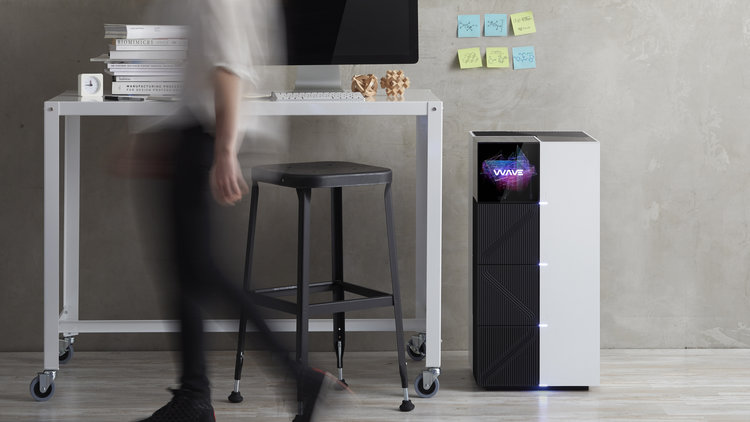
\includegraphics[trim=0cm 0cm 0cm 0cm, clip=true,scale=1]{figures/wave_lab.jpg}
    \caption{Wave Consumer Unit\label{Fig:wavelab}}\vspace{-4mm}
    \end{figure}

\subsection*{MIPS Acquisition}
\paragraph{}
MIPS is one of the old time giants of the silicon design game. To facilitate their ideology of integrating dataflow technology to small devices, Wave Computing recently acquired MIPS~\cite{mipsaq} for their silicon design expertise. With this step, Wave computing hopes to realize their idea of "Bringing datacenter to the edge" by installing datacenter level high performance hardware in small(edge) devices.

\subsection{Company History - Paraqum Technologies}
\paragraph{}
Started in 2013 as a continued final year project of four students from the 2008 batch of University of Moratuwa Department of Electronic and Telecommunication Engineering, Paraqum Technologies was first located inside the university itself. The CEO also being a lecturer in the University, this was the result of the attempt to promote technical entrepreneurs to rise up from the university level.

\paragraph{}
Paraqum Technologies quickly developed into a full sized technology startup and by 2018, the staff had grown to around 40 and every year they took around 10-12 interns under their wings to properly expose them to the electronic industry. Now they have design contracts from renowned industrial leaders and their own networking product line which is also very famous for their unique capabilities.

\begin{figure}[h]
    \centering
    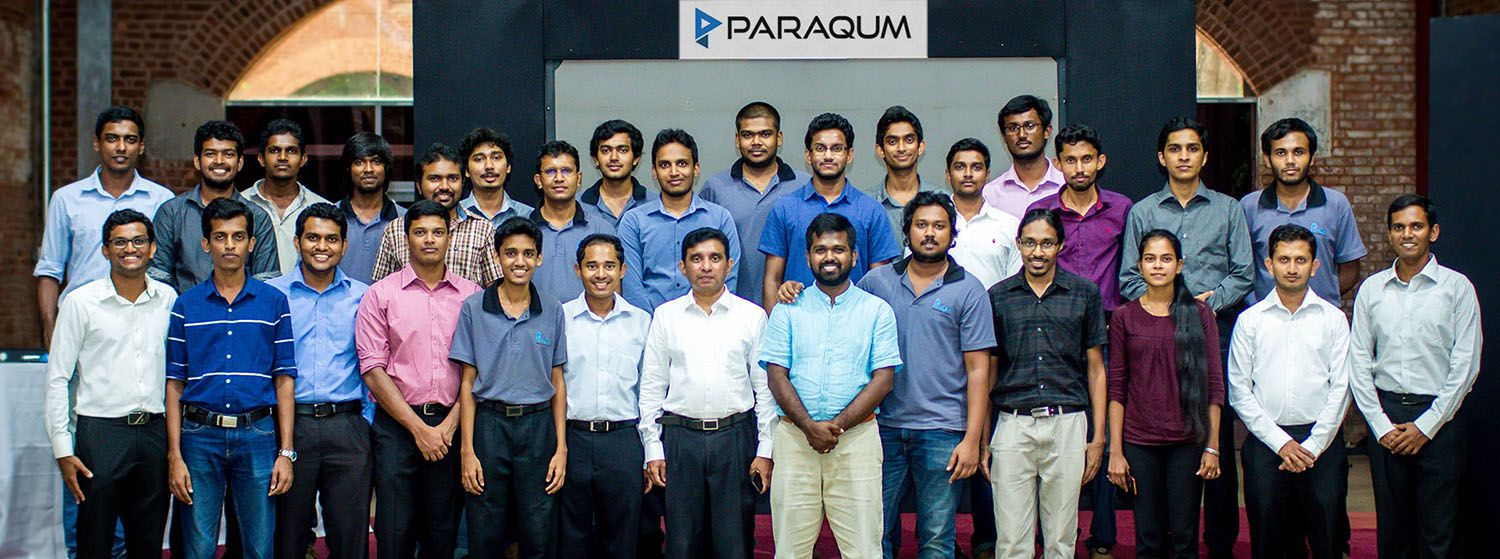
\includegraphics[trim=0cm 0cm 0cm 0cm, clip=true,scale=0.25]{figures/paraqum_team.jpg}
    \caption{Paraqum Technologies Staff (including Wave team members)~\cite{pqmintro} \label{Fig:pqmteam}}\vspace{-4mm}
    \end{figure}

\subsection{Wave-Paraqum partnership, separation and its effect on interns}

\paragraph{}
As described above, Paraqum Technologies had a design contract from wave computing for their toolchain and application needs. This contract had been in place for almost two years and has proved to be one of the most productive teams wave computing has ever employed. They have helped in designing the hardware part of the dataflow processing chips and by the time we started our internships, they were working on RTL level software projects.

\paragraph{}
However, Wave computing had decided it would be better to acquire the Sri Lankan team for themselves. So, in november 2018, the Wave Computing team was separated from Paraqum Technologies and established as the Sri Lankan branch of Wave Computing (pvt) ltd. with no connection to Paraqum Technologies whatsoever. Before Separation, Wave computing team worked in the Paraqum Technologies office in Kohuwala but after that they moved to a new office in Bambalapitiya.

\begin{figure}[h]
    \centering
    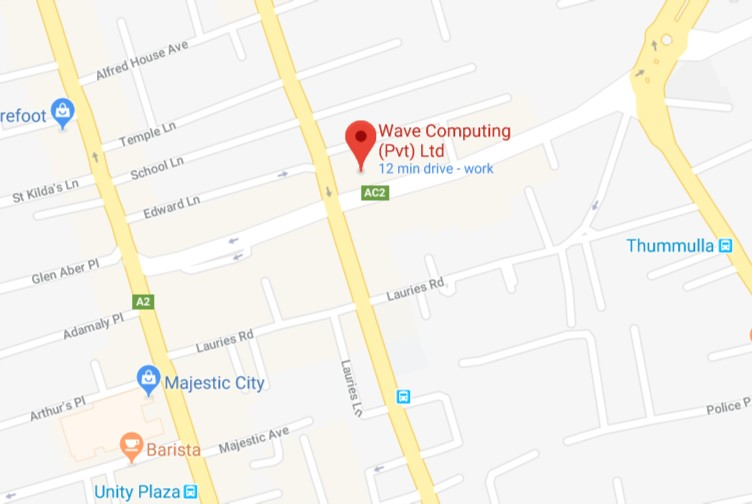
\includegraphics[trim=0cm 0cm 0cm 0cm, clip=true,scale=0.25]{figures/wave_location.jpg}
    \caption{Wave Computing Office location \label{Fig:pqmteam}}\vspace{-4mm}
    \end{figure}

\paragraph{}
As the organizations separated, interns of the wave team also moved to work in the new office premises and work was carried out as normal. But the internship contracts were not changed and technically, we were interns of Paraqum Technologies for the whole 24 weeks but worked under the supervision of Wave Computing staff. Therefore this report will be more focused on Wave Computing.

\subsection{Organization Structure and Hierarchy}

\paragraph{}
Wave computing team was another division in Paraqum Technologies until the separation but after that they became a fully independent entity. The dotted line in the following diagram represents the administration link that existed before the separation. Now Wave computing Sri Lanka operates directly under the administration of their head office in Campbell, California. 

\begin{figure}[h]
    \centering
    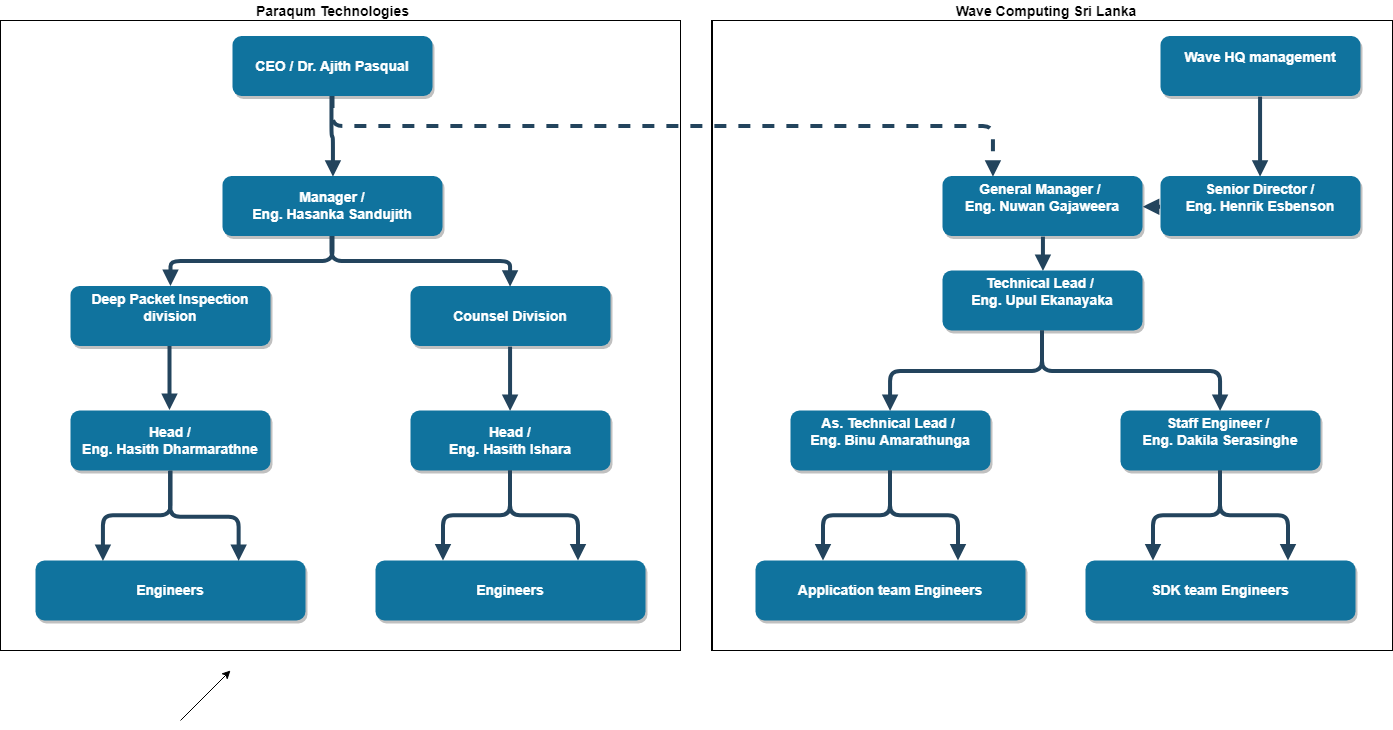
\includegraphics[trim=0cm 0cm 0cm 0cm, clip=true,scale=0.25]{figures/admin_struct.png}
    \caption{Wave/Paraqum administration structure \label{Fig:adminstruct}}\vspace{-4mm}
    \end{figure}

\subsection{Areas of Interest}

\begin{figure}[h]
    \centering
    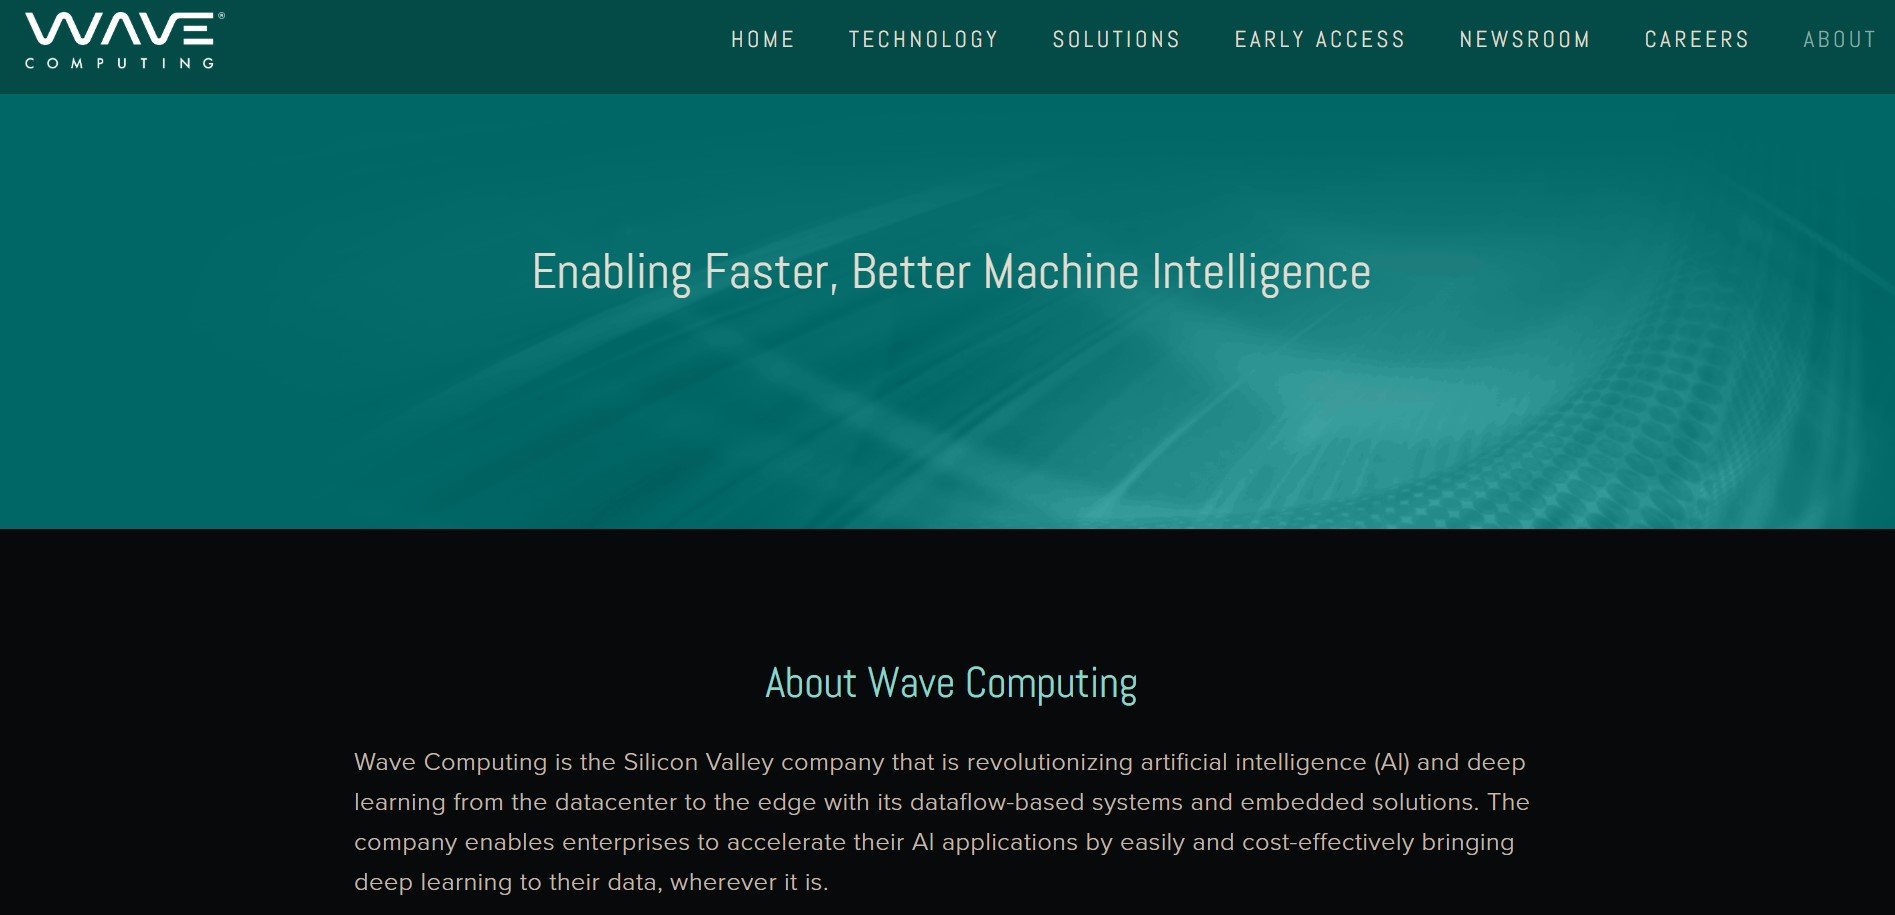
\includegraphics[trim=0cm 0cm 0cm 0cm, clip=true,scale=0.25]{figures/wave_site.jpg}
    \caption{Wave computing Homepage with their target of better AI\label{Fig:wavesite}}\vspace{-4mm}
    \end{figure}

\paragraph{}
The main focus of Wave computing is to Introduce new processing system for heavy computational operations with their proprietary dataflow processing technology. When the system is built and released, it can be used for:

\subsubsection*{Artificial Intelligence}
\paragraph{}
The main use of the dataflow processing units (DPU) is intended to be Artificial Intelligence systems. Current hardware in our devices are not suited for the massive amount of data that need to be processed in parallel. The DPU has been optimized for this particular task to perform it at high speed. It is speculated that once wave DPU systems become available in market, it will spark a revolution in the AI industry.

\subsubsection*{Edge devices}
\paragraph{}
Edge devices are small devices such as mobile phones and IoT sensors. Wave computing already has plans in motion to develop high performance, small size hardware to be installed in these edge devices. This will allow us to have very powerful yet small devices for our day to day usage.

\subsubsection*{Image processing}
\paragraph{}
Image processing and AI are similar in many ways. The parallel data handling capacity of DPU systems makes it an ideal candidate for image processing applications such as self driving or biometric authentication.


\subsection{DARPA Subterranean Challenge}
\label{ssec:darpa}
\paragraph{}
The RAG of CSIRO was recently selected as one of the six funded teams worldwide for the DARPA Subterranean Challenge \cite{darpa} by United States Department of Defense. Therefore the next four years of research in Robotics in CSIRO will be more focused on developing robots that can simultaneously map and navigate complex environments such as underground tunnels, caves and mines without GPS or reliable communication with humans. It is an ideal project for DATA61, where their experience and expertise in SLAM, Hovermap and legged robots come together. By investing in this project for the next few years, DATA61 aims to develop new technology that can be later commercialized into different applications. 

%Image: Darpa challenge
\begin{figure}[H]
    \centering
    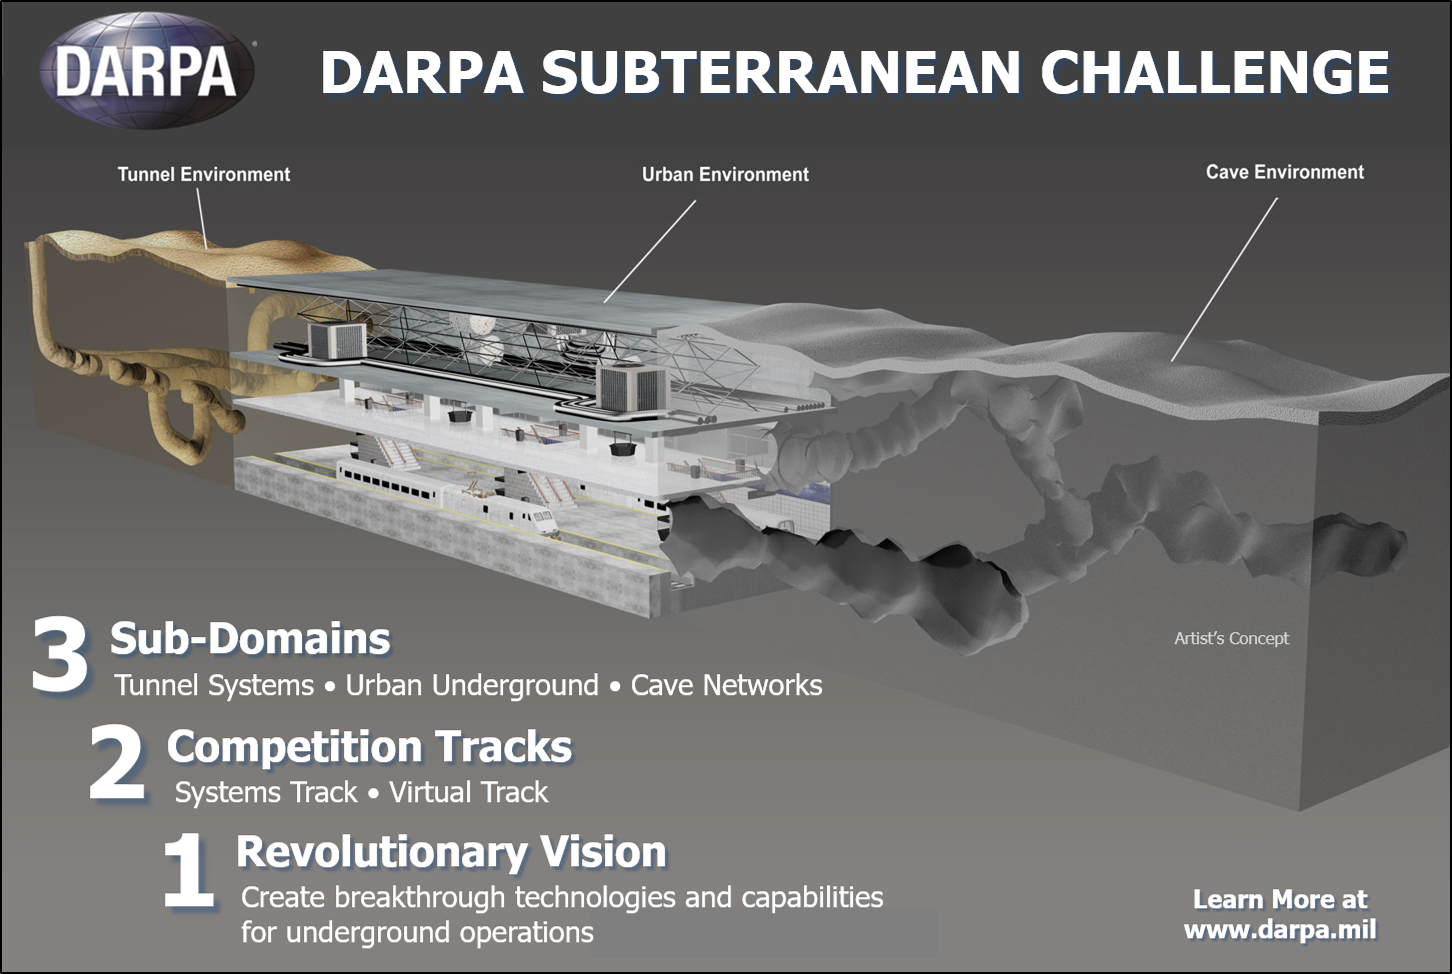
\includegraphics
        [width=12cm]
        {figures/subt_challenge.png}
    \caption{CSIRO focuses on DARPA challenge}\vspace{-4mm}
\end{figure}

\paragraph{}
This is the second competition held by DARPA to encourage development of cutting edge technology around the world. The first DARPA Robotics Challenge was held from 2012-2015 where the goal was to build a robot that can navigate a disaster site and perform tasks like driving a car, opening a door, drilling into the wall and so on, with an unreliable communications connection with the controlling humans. In case of future disasters like Fukushima Nuclear disaster, where humans cannot approach the site due to radiation, such robots can be utilized. The second competition focuses on subterranean environment, with the goal of buildings robots that can navigate the drug trafficking, human trafficking tunnels and save people stuck in mines and underground caves.

\paragraph{}
For this task, incorporating machine learning into the workflow of algorithm development and testing is of paramount importance for all researches in RAG. I addressed this problem by developing an efficient end-to-end pipeline for this and demonstrating it through two projects.


\subsection{Current Situation}
\paragraph{}
After years of research, development and commercialization of projects, DATA61 has risen as a world leader in many of their technologies. Hundreds of papers have been published from DATA61 in the past and are being published into reputed journals. Currently, DATA61 is being restructured and some of the technologies developed there have evolved into successful startup companies.

\subsection{Impacts on Sri Lankan Industry}
\paragraph{}
Being a part of the national research institute of Australia, DATA61 does not directly contribute to the Sri Lankan industry. However the research that is published in public domain can be used by Sri Lankan companies for their research and development.

\newpage
\subsection{SWOT Analysis}

\subsubsection*{Strengths}
\paragraph{}
DATA61 has ample resources and funds for its research programs. As a result a multitude of projects are being executed. Also the work culture in CSIRO encourages cross pollination of ideas and creativity. Their inclusive policy allows students and researchers from all around the world to come together and share their expertise and experience.

\subsubsection*{Weaknesses}
\paragraph{}
Although almost all researchers are friendly and helpful to each other, due to the way projects are assigned and due to the management structure, most of them work alone on a project. This has led to fragmentation, where people working on similar projects are unable to cooperate better. This is now addressed through weekly group meetings for Robotics, Machine Learning and standardization of the workflow, hardware and software APIs used in different projects.


\subsubsection*{Opportunities}
\paragraph{}
Being recognized as the world leader in their technologies, DATA61 has the opportunities to collaborate with other world class research institutes such as NASA Jet Propulsion Laboratory and ETH. We had the chance to attend lectures and discussions done by researchers from these institutes during our internship period. Also, DATA61 attracts talent from around the world and from within Australia, which would help them in the future research.

\subsubsection*{Threats}
\paragraph{}
DATA61 is a research organization that is funded for research that empowers the Australian industries. However, in the meanwhile they need to invest in pure science research the outcomes of which cannot be known in advance. This balance of funding projects of pure and applied science is vital to the success of DATA61 as an organization. If most of its research does not produce marketable technology, DATA61 is in danger of being under-funded by the australian government, meanwhile focusing more into applied science is not a sustainable strategy. This issue was discussed on multiple meetings as a part of their restructuring process.


\subsection{Usefulness to the Country}
\paragraph{}
DATA61 and CSIRO are important pillars of the Australian economy and society. The technologies materialized in DATA61 have laid the foundations for many companies in their industry and several companies collaborate with DATA61, paying them to use their service. This creates a win-win equilibrium that is beneficial to all parts of the economy.

\paragraph{}
Also, their research in healthcare, data privacy and infrastructure has been helping the australian society for the past few years. Their research into livestock management using IOT is helping the agriculture-based economy of the Queensland state. Hovermap and their research in mining is used to find new mineral deposits and analyze their composition. DATA61 is also modelling and devising algorithms to control traffic in different cities of Australia. 

\subsection{Suggestions to Improve the Company}
\begin{itemize}
    \item Implement a better project management system for intern students.
    \item Assign supervisors and well-defined projects that are compatible with the skills of students.
    \item Set deadlines for the student interns and monitor the progress.
    \item Provide concessions for students who live far away, as the public transport is considerably expensive.
\end{itemize}